%このファイルは、表紙を結合したPDFファイルを作るためのもの。
%bash zentai.command を実行することで
%まず、main.texをplatexで処理し、次にkanse.texがpdfLaTeXで処理されて
%hyosi.pdf+ryonaitizu.pdf+main.pdfという風に結合されたkanse.texができる。

%表紙は色紙に別刷りなので、本番ではこれは使わない。

\documentclass[flegn]{article}
\usepackage{pdfpages}
\begin{document}

\includepdf[pages=-,noautoscale=true, scale=1.0]{hyosi.pdf}
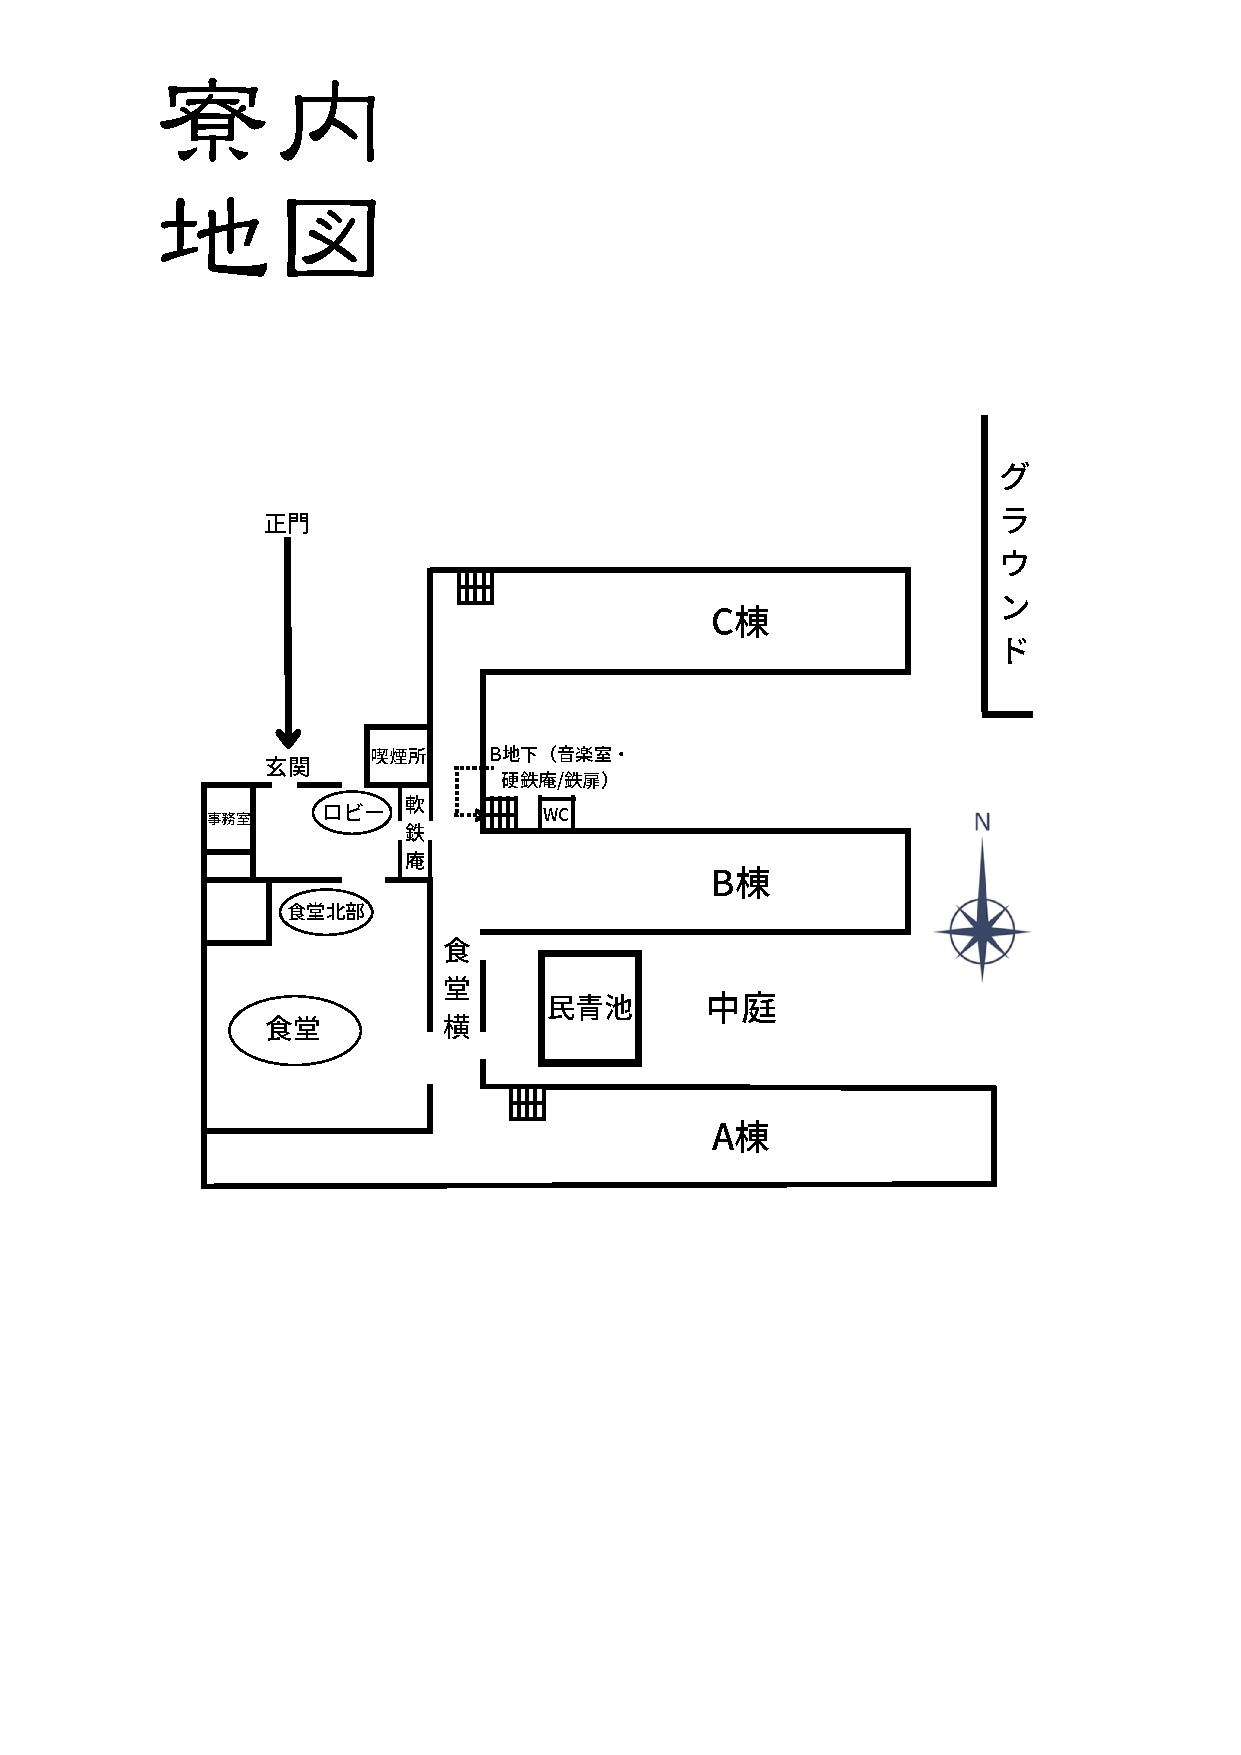
\includepdf[pages=-,noautoscale=true, scale=1.0]{ryonaitizu.pdf}
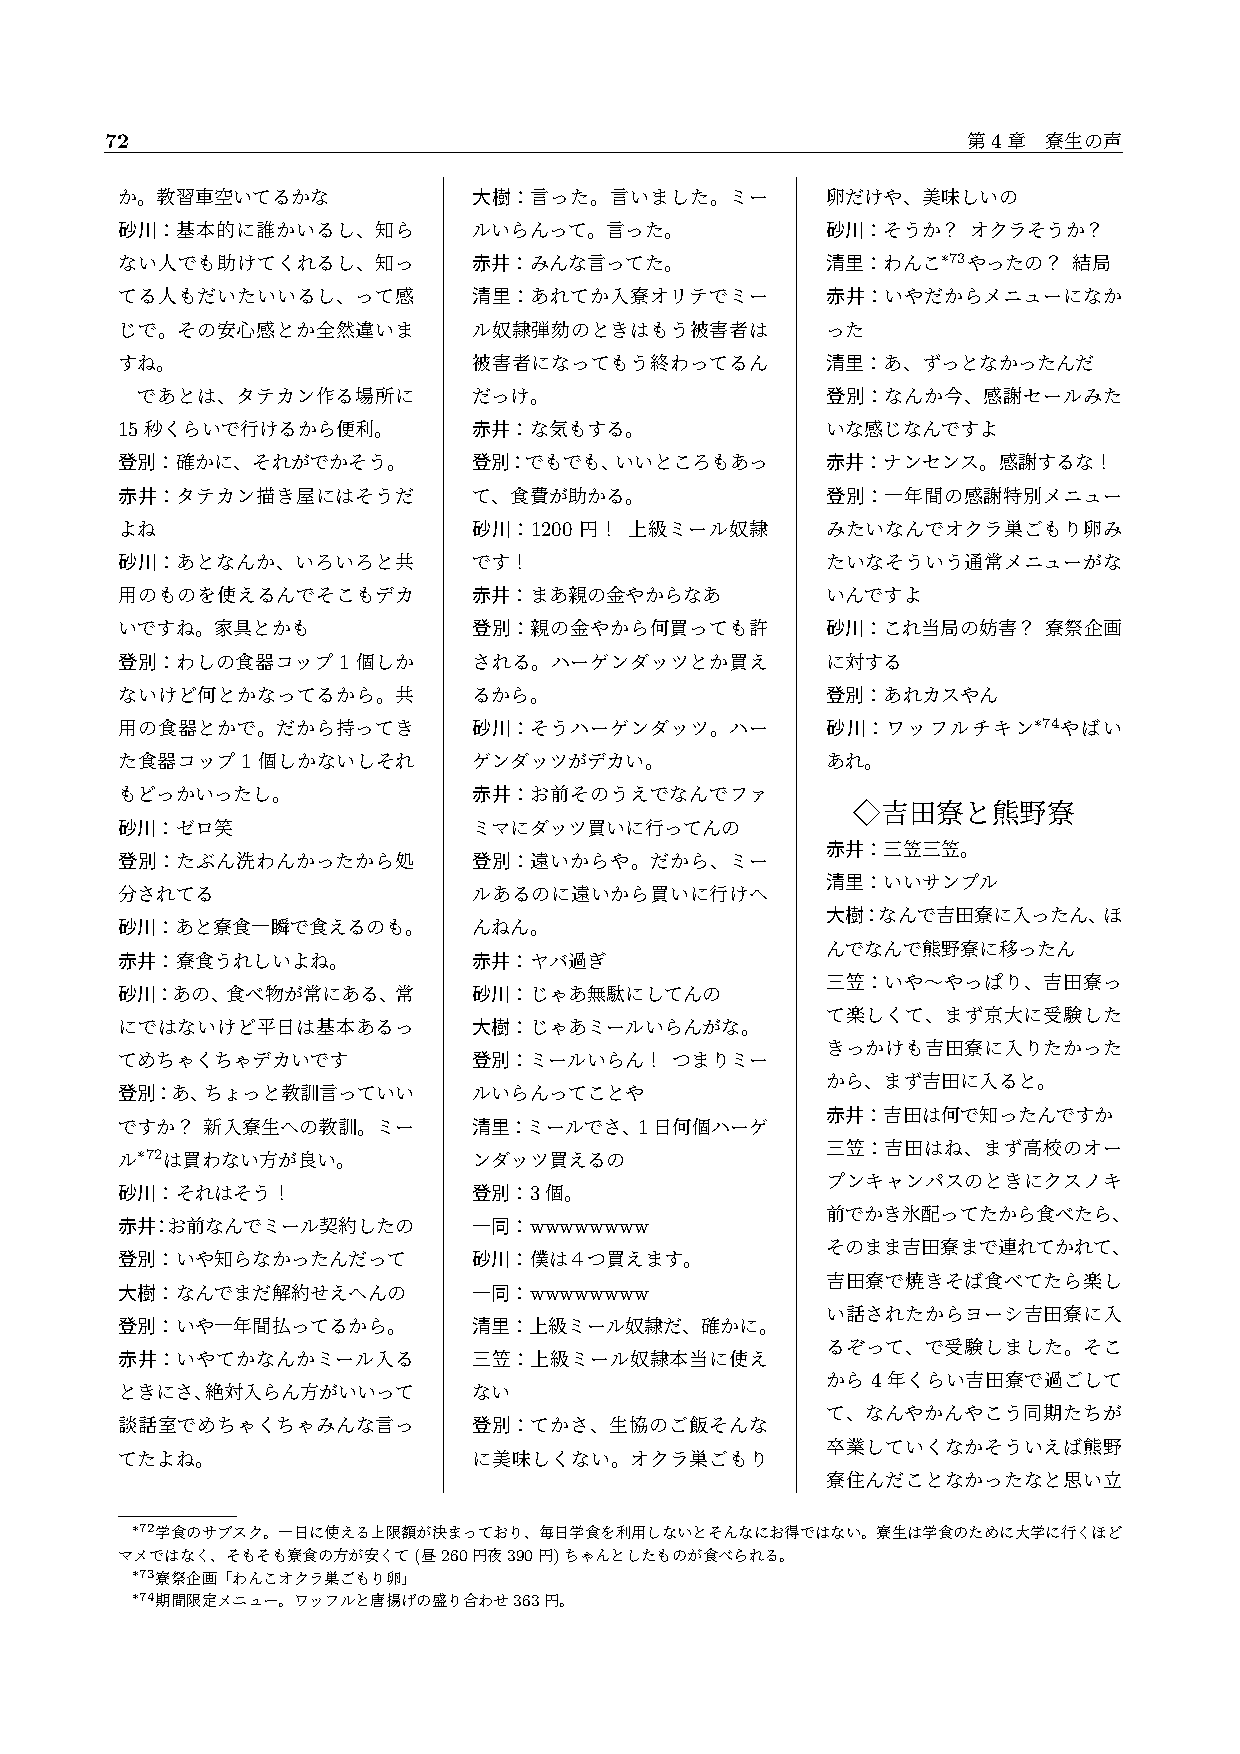
\includepdf[pages=-,noautoscale=true, scale=1.0]{main.pdf}
\end{document}